\documentclass{article}

\usepackage{times}
\usepackage{geometry}
\geometry{a4paper,left=0.6cm,right=0.7cm,top=2cm,bottom=1cm,columnsep=0.8cm}
\usepackage{fontawesome}
\usepackage[hidelinks]{hyperref}
\usepackage{multicol}
\usepackage{tikz}
\usepackage{hyphsubst}
\usepackage{moresize}
\usepackage{hyphenat}
\usepackage{tabularx}
\usepackage{xcolor}
\usepackage{enumitem}

\newcolumntype{Y}{>{\RaggedRight\arraybackslash}X}

\setlist[itemize]{itemsep=1pt,leftmargin=*,topsep=-10pt}

\definecolor{maincolor}{HTML}{f0fafc}
\definecolor{seccolor}{HTML}{ffffff}
\definecolor{gray}{HTML}{8c94a9}
\definecolor{sidetext}{HTML}{59cee5}

\usepackage[contents={}]{background}
\AddEverypageHook{\begin{tikzpicture}[remember picture,overlay]%
  \node[inner sep=0pt,outer sep=0pt] at (current page.north west) [anchor=north west]{%
  \fcolorbox{maincolor}{maincolor}{%
\begin{minipage}[t][\paperheight][t]{0.3\paperwidth}
        \color{white}
        \hspace{0.08cm}
\end{minipage}}
\fcolorbox{seccolor}{seccolor}{
\begin{minipage}[t][\paperheight][t]{0.67\paperwidth}
        \color{black}
        \hspace{1cm}
\end{minipage}
}
  };%
\end{tikzpicture}
}

\setlist[itemize]{itemsep=-2pt,topsep=0pt,leftmargin=1.08cm}
\renewcommand{\labelitemi}{\textcolor{sidetext}{\footnotesize$\bullet$}}

\setlength{\parindent}{0pt}
\usepackage{paracol}

\begin{document}

\pagestyle{empty}

\columnratio{0.3}
\begin{paracol}{2}
\color{sidetext}
\begin{center}
            \begin{tikzpicture}
            \clip (0,0) circle (1.5cm) node[anchor=center] {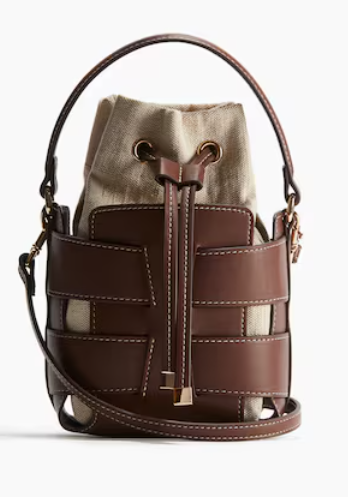
\includegraphics[width=3cm]{595f22f0dd2448f2b625fe1422f808a1.png}}; 
            \end{tikzpicture}

            ~

         {\color{black}\LARGE \textbf{Pape Saliou FALL}}

         ~

         {\large{Data Scientist}}

        
        \end{center}

{\color{gray}\rule{\linewidth}{0.4pt}} \\

 \begin{tabular}{cl}
            \faPhone{}      & 
            \begin{tabular}{p{0.7\linewidth}}
            {\color{gray}Téléphone}\\
            {0753481453}
            \end{tabular}
            \\ \\
               \faLinkedin{}      & 
            \begin{tabular}{p{0.7\linewidth}}
            {\color{gray}LinkedIn}\\
            {\href{https://www.linkedin.com/in/}{https://www.linkedin.com/in/}}
            \end{tabular}
            \\ \\
               \faMapMarker{}      & 
            \begin{tabular}{p{0.7\linewidth}}
            {\color{gray}Adresse}\\
            {Paris, France}
            \end{tabular}
            \\ \\
               \faEnvelope{}      & 
            \begin{tabular}{p{0.7\linewidth}}
            {\color{gray}Email}\\
            {\href{mailto:zine@prepaya.fr}{zine@prepaya.fr}}
            \end{tabular}
            \\
        \end{tabular}
        \vspace{.2cm} \\
        {\color{gray}\rule{\linewidth}{0.4pt}} \\

        {\color{black}{Langues}}

        ~
        
        \begin{tabular}{cl}
            {\Large\faLanguage{}} & \begin{tabular}{l}
             Français \textendash{} Natif\\
             Anglais \textendash{} Courant
            \end{tabular} \\
        \end{tabular}
        \vspace{10pt} \\
        {\color{gray}\rule{\linewidth}{0.4pt}} \\

        \vspace{.4cm}

        {\color{black}{Compétences clés}}

        ~
        
        \begin{tabular}{ll}
         \begin{minipage}{0.1\linewidth}
         
\includegraphics[width=\linewidth]{picon.png}
         \end{minipage} & Python \\[10pt]
         \begin{minipage}{0.1\linewidth}
         
\includegraphics[width=\linewidth]{picon.png}
         \end{minipage} & R \\[10pt]
         \begin{minipage}{0.1\linewidth}
         
\includegraphics[width=\linewidth]{picon.png}
         \end{minipage} & SQL \\[10pt]
         \begin{minipage}{0.1\linewidth}
         
\includegraphics[width=\linewidth]{picon.png}
         \end{minipage} & Machine Learning \\[10pt]
         \begin{minipage}{0.1\linewidth}
         
\includegraphics[width=\linewidth]{picon.png}
         \end{minipage} & Deep Learning \\[10pt]
        \end{tabular}
        
\switchcolumn
\color{black}

\textcolor{black}{\Large \textbf{Profil Professionnel}} \\

Data Scientist avec plus de 3 ans d’expérience dans la conception de modèles prédictifs, l’analyse statistique et la valorisation des données. Passionné par la résolution de problèmes complexes, je mets la science des données au service des enjeux business pour générer de la valeur mesurable.\\[8pt]

\textcolor{black}{\Large \textbf{Expérience Professionnelle}} \\

\colorbox{maincolor}{%
  \begin{minipage}{\linewidth}
    \begin{tabular}{@{}lp{0.72\linewidth}r}
      \begin{minipage}{0.05\linewidth}
        
\includegraphics[width=\linewidth]{picon.png}
      \end{minipage} & 
      qsksbkcbkSB &  
      {\footnotesize 2022-01 -- 2023-12 } \\[-10pt]
      & {\color{sidetext}{Data Scientist}} & \\
      & {\small Paris, France } & \\
    \end{tabular}
\begin{itemize}
    \item Conçu et déployé des modèles de machine learning pour prédire le churn client (+15\% de précision).
    \item Automatisé les pipelines de données en Python (Airflow) réduisant le temps de traitement de 40\%.
    \item Réalisé des visualisations interactives sous Power~BI pour guider les décisions métier.
    \item Collaboré avec les équipes produit et marketing pour transformer les insights en actions.
    \item Mis en place des tests A/B et évalué les performances des modèles.
\end{itemize}
  \end{minipage}%
}

\vspace{1cm}

\textcolor{black}{\Large \textbf{Formation}} \\[2pt]

 \begin{tabular}{@{}cp{0.7\linewidth}}
      \begin{minipage}{0.05\linewidth}
        
\includegraphics[width=\linewidth]{picon.png}
      \end{minipage} & \vspace{-12pt}
      {\color{sidetext} Master 2 Data science} \\[-6pt]
      & Sorbonne Université \\[-6pt]
      & 2012--2015 
    \end{tabular}

\vspace{0.5cm}

\textcolor{black}{\Large \textbf{Certifications}} \\

\begin{itemize}[leftmargin=12pt]
\item ksLD  -- KSLQKBC (Jul-2024)
\end{itemize}

\end{paracol}



\end{document}